\documentclass[slidestop,compress,mathserif,10pt]{beamer}

\mode<article> % 仅应用于article版本
{
  \usepackage{beamerbasearticle}
%  \usepackage{fullpage}
  \usepackage{hyperref}
}

%% 下面的包控制beamer的风格,可以根据自己的爱好修改
\usepackage{beamerthemesplit}   % 使用split风格
\usepackage{beamerthemeshadow}  % 使用shadow风格
%\usepackage[width=2cm,dark,tab]{beamerthemesidebar}
%\usepackage{beamerthemetree}
%\usetheme{Montpellier}
%\usecolortheme{lily}


%% 这些包是可能会用到的,不必修改
\usepackage{amsmath,amssymb}
\usepackage{graphicx}
%\usepackage{color}
%\usepackage{pgf,pgfarrows,pgfnodes,pgfautomata,pgfheaps}
%\usepackage{multimedia}

%\documentclass{beamer}
%\usepackage{beamerthemeshadow}
\usepackage{beamerthemesplit}
%\usetheme{shadow}
\usepackage{graphicx}
\usecolortheme{lily}
%\usepackage{amsmass}
\usepackage{amssymb,amsfonts,url}
\graphicspath{{Problems/}}

%\usepackage{CJK}
%\usepackage{pinyin}

%    \begin{figure}
%        \centering
%        \includegraphics[width=0.8\textwidth]{newGeneRep.eps}
%    \end{figure}

% \begin{figure}%
%   \begin{center}%
%     \begin{minipage}{0.70\textwidth}%
%      \includegraphics[width=1.0\textwidth]{comp25000.eps}%
%     \end{minipage}%
%     \begin{minipage}{0.30\textwidth}
%      \includegraphics[width=1.0\textwidth]{comparelabel.eps}%
%     \end{minipage}%
%   \end{center}
% \end{figure}

% \begin{table}
%   {\begin{tabular}{l|rrr}\hline
%       & \multicolumn{3}{c}{Actual number of DCJ operations}\\
%       \# genes &\# genes $\times 1$&\# genes $\times 2$&\# genes  $\times 3$ \\
% \hline
%      (a)~25,000 & 0.5\% ~~&  0.9\% ~~& 1.7\%~~\\
%       (b)~10,000 & 0.8\%~~ &  1.4\% ~~& 2.7\%~~\\
%      (c)~ 1,000 & 2.7\%~~ & 4.7\%~~ & 14.7\%~~\\ \hline
%     \end{tabular}} {}%
% \end{table}

% \begin{eqnarray}
% T(n) &=&  \sum\nolimits_{i=1}^n C_i \\
%      &=&  \# PUSH + \#POP \\
%      &<& 2\times \#PUSH \\
%      &<& 2n \\
% \end{eqnarray}

% \[ 
% \begin{matrix}
% \begin{pmatrix}
% C_{11} & C_{12} \\ 
% C_{21} & C_{22} 
% \end{pmatrix}
% =
% \begin{pmatrix}
% A_{11} & A_{12} \\ 
% A_{21} & A_{22}  
% \end{pmatrix}
% 
% \begin{pmatrix}
% B_{11} & B_{12} \\ 
% B_{21} & B_{22}  
%  
% \end{pmatrix}
%     
%    \end{matrix}
% \]
% 
% 
% \begin{eqnarray}
%  C_{11} &=& (A_{11}\times B_{11}) + (A_{12} \times B_{21}) \\
% C_{12} &=& (A_{11}\times B_{12}) + (A_{12} \times B_{22}) \\
% C_{21} &=& (A_{21}\times B_{11}) + (A_{22} \times B_{21}) \\
% C_{22} &=& (A_{21}\times B_{12}) + (A_{22} \times B_{22}) 
% \end{eqnarray}
% \begin{figure}%
%      \begin{minipage}{0.32\textwidth}%
%       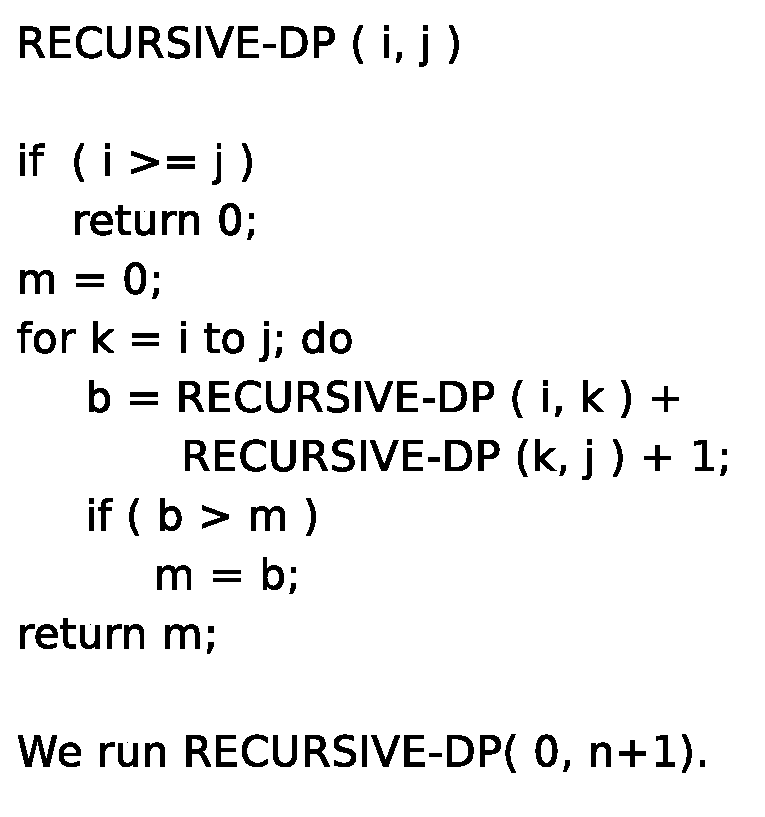
\includegraphics[width=1.0\textwidth]{L7-intervalschedulingdpalgo.eps}%
%      \end{minipage}%
%  \quad
%      \begin{minipage}{0.30\textwidth}
%       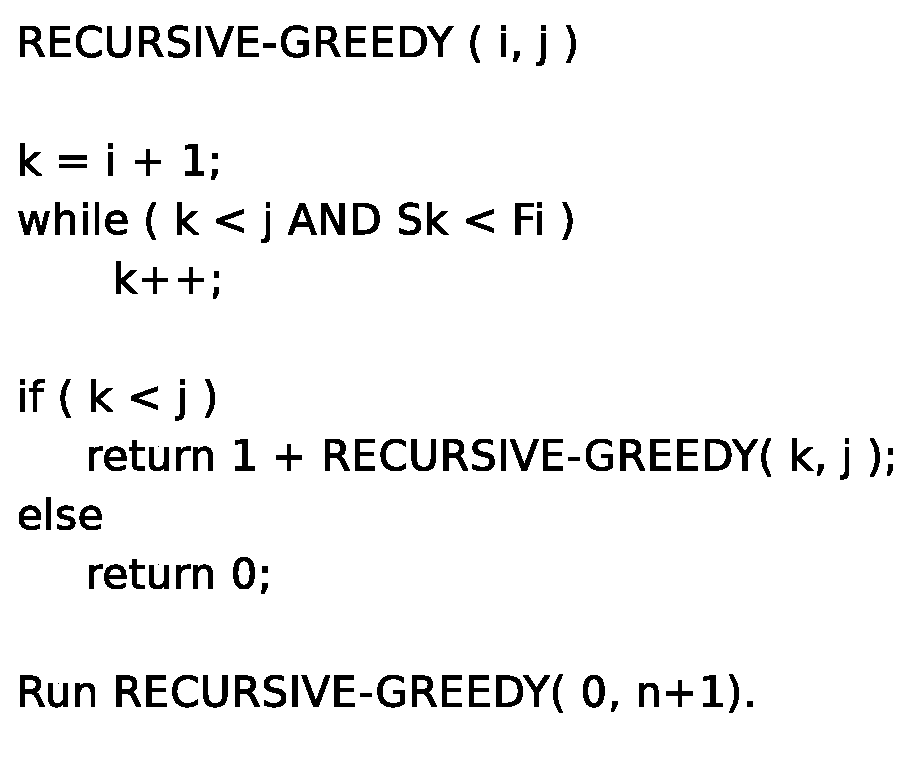
\includegraphics[width=1.0\textwidth]{L7-intervalschedulinggreedyalgo.eps}%
%      \end{minipage}%
%  \quad
%       \begin{minipage}{0.25\textwidth}
%       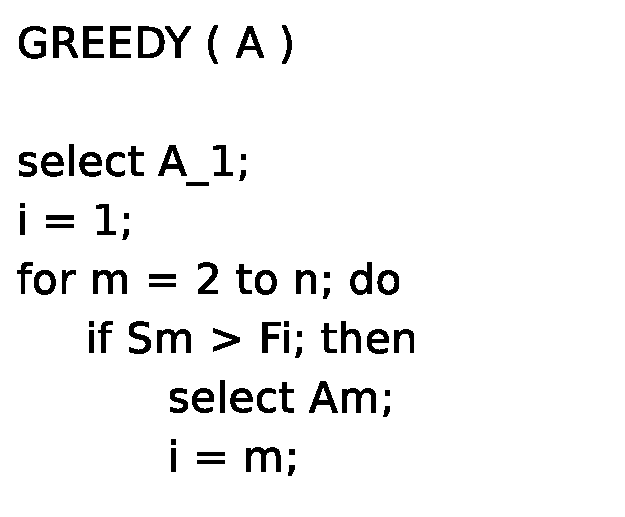
\includegraphics[width=1.0\textwidth]{L7-intervalschedulinggreedyalgo2.eps}%
%      \end{minipage}%
% 
%  \end{figure}

\title{CS612  Algorithm Design and Analysis }
\subtitle{ Lecture 17. String matching 
\footnote{The slides are made based on Randomized Algorithm by R. Motwani and P. Raghavan, http://www-igm.univ-mlv.fr/~lecroq/string/, and a lecture by T. Chan. } }
\author{Dongbo Bu \\
\ \\
{\small Institute of Computing Technology \\ 
Chinese Academy of Sciences, Beijing, China}}

\date{}

\begin{document}
%\begin{CJK}{UTF8}{cyberbit}

\frame[allowframebreaks]{\titlepage}

\frame[allowframebreaks]{
\frametitle{Outline}
\begin{itemize}
\item Introduction
\item DFA and KMP methods 
\item A Monte Carlo method 
\item Rabin-Karp randomized algrorithm; 
\end{itemize}
}

\frame[allowframebreaks]
{
\frametitle{ {\sc StringMatching} problem }

\begin{block}{}
{\bf INPUT: } \\
Given strings $t=t_1t_2...t_n$,$(t_i \in \{0,1\}, i=1,2,...,n)$ and $p=p_1p_2...p_m$, $(p_j \in \{0,1\}, j=1,2,...,m)$, $m\leq n$; \\
{\bf OUTPUT: }\\ Is $p$ a substring of $t$? 
\end{block}

$t$ is called ``text'' and $p$ is called ``pattern''.
}

\frame{
\frametitle{ DFA-based methods }
\begin{itemize}
 \item Brute-force method: checking every possible occurence of $p$ in $t$. Time-complexity: $O(nm)$ (when searching for $a^{m-1}b$  in $a^n$ for instance.) 
 \item DFA-based method: 
 \begin{enumerate}
  \item building a DFA for all string containing $p$;
  \item running this DFA on $t$; 
  \item Time-complexity: $O(f(m) + n)$. Here, $f(m)$ denotes the time to build a DFA. It is possible that $f(m)=O(m)$. 
  \end{enumerate}
\end{itemize}
e.g.: $p=101$
\begin{figure}
        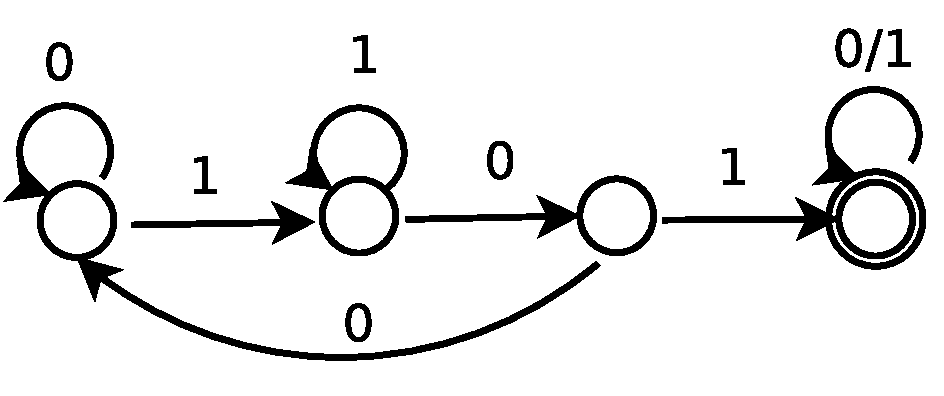
\includegraphics[width=2.5in]{L14-DFA101.eps}
\end{figure}
}

\frame{
\frametitle{ KMP and BM algorithms }
\begin{enumerate}
 \item Karp-Morris-Parrat method: \\
\begin{itemize}
\item Similar to DFA but with a ``compressed'' representation of DFA. 
\begin{figure}
        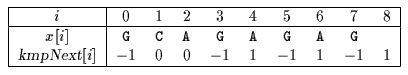
\includegraphics[width=2.5in]{L14-KMPtable.eps}
\end{figure}
\end{itemize} 

 \item Boyer-Moore method:  \\
\begin{itemize}
\item The Boyer-Moore algorithm is considered as the most efficient string-matching algorithm in usual applications. 
\item The algorithm scans the characters of the pattern from right to left beginning with the rightmost one. In case of a mismatch (or a complete match of the whole pattern) it uses two precomputed functions to shift the window to the right. These two shift functions are called the good-suffix shift (also called matching shift and the bad-character shift (also called the occurrence shift).
\end{itemize}
\end{enumerate}
}

\frame[allowframebreaks]{
\frametitle{ An interesting sub-problem }

Problem:
\begin{itemize}
 \item Alice has a string $u$, and Bob has a string $v$, $u, v \in \{0,1\}^*$, $|u|=|v|=n$.
 \item They want to see whether $u=v$.
\end{itemize}

Possible ways:
\begin{enumerate}
 \item transmit $n$ bits; 
 \item transmit a ``fingerprint'' with $O( d \log n )$ bits; 
\end{enumerate}

}
\frame[allowframebreaks]{
A randomized finger-print: 
\begin{itemize}
 \item Let $x=\{0,1,...,P-1\}$, where $P$ is a large prime number;
 \item Define a finger-print $F_x: \{0,1\}^* \rightarrow \{0,1,2,...,P-1\}$ as follows: \\
 \qquad $F_x(a_{n-1}a_{n-2}...a_0) = \sum_i a_i x^i \mod P$.  
\end{itemize}

Monte-Carlo algo: 
\begin{enumerate}
 \item $x=random(0, P-1)$, where $P$ is a large prime number;
 \item Alice transfers $F_x(u)$ to Bob;
 \item Bob calculate $F_x(v)$ first, and reports ``Yes'' if $F_x(u)=F_x(v)$; Otherwise reports ``No'' (definitely ``No'').
\end{enumerate}

Error analysis: 
\begin{enumerate}
 \item Case 1: ($u=v$). Correct.
 \item Case 2: ($u\neq v$) Error: Bob reports ``Yes'', i.e., $F_x(u)=F_x(v)$ when $u\neq v$. 
\begin{eqnarray}
 & & \Pr ( F_x(u) = F_x(v) | u \neq v )  \nonumber \\ 
&=& \Pr ( \sum_{i=0}^{n-1} u_i x^i = \sum_{i=0}^{n-1} v_i x^i \mod P ) \nonumber\\
&=& \Pr ( \sum_{i=0}^{n-1} ( u_i - v_i ) x^i = 0 ) \nonumber \\
&\leq& \frac{n-1}{P} \quad \text{ by Fact 1.} \nonumber 
\end{eqnarray}
 \item $\Pr ( F_x(u) = F_x(v) ) \leq \frac{1}{n^d}$ when setting $P=n^{d+1}$. 
\end{enumerate}
Fact 1: \\
   A polynomial of degree $\leq n-1$ has at most $n-1$ roots $\mod P$. 
}

\frame[allowframebreaks]{
\frametitle{ Rabin-Karp randomized algorithm for string matching. }
\begin{itemize}
 \item Rabin-Karp Algo ($s, t$): 
\begin{enumerate}
 \item $x=random(0, P-1)$; 
 \item $A = F_x(s_0s_1...s_m)$, $B=F_x(t_0t_1...t_m)$; \\
 \item for $i=0$ to $n-m$ \\
 \item   \qquad //compare $s_{i+1}s_{i+2}...s_{i+m}$ with $t_1t_2...t_m$; 
 \item   \qquad  $A = ( A - a_{i+1}x^m ) x + a_{i+m+1} \mod P$; 
 \item   \qquad  if ( $ A == B $ ) return ``possibly match'';
 \item return ``No''; 
\end{enumerate}
\item Time-complexity: $O(n)$. 
\item Error probability: 
\begin{enumerate}
 \item Let $E_i$ denote the event: algo errs at the $i$-th iteration. We have: \\
 \item $\Pr( E_i ) \leq \frac{m-1}{P}$ \\
 \item $\Pr( Error ) = \Pr( \cup_{i=0}^{n-m} E_i ) \leq \sum_i \Pr(E_i) \leq \frac{nm}{P} \leq \frac{n^2}{P}$ 
 \item $\Pr( Error ) \leq \frac{1}{n^d}$ by setting $P=n^{d+1}$.
\end{enumerate}
\end{itemize}

}

\frame{
\frametitle{A Las Vegas version}

Algo: 
\begin{enumerate}
 \item Run Karp-Rabin; \\
 \item if it returns ``No'', returns ``No'';
 \item else 
 \item \qquad    Verify $s = t$ ;
 \item \qquad    if so, return ``Yes''; else goto Step 1;  
\end{enumerate}

Analysis: 
\begin{itemize}
 \item If Karp-Rabin is correct: $O(n)$ time is enough;
 \item otherwise, the execution of brute-force algo costs $O(mn)$ time.
\end{itemize}
Expected running time:
$E(T) = O(n) ( 1 - \frac{1}{n^d} ) + O(mn) \frac{1}{n^d}  = O(n)$. (setting $d=1$)
} 


\end{document}
